\documentclass[aspectratio=169,11pt]{beamer}
\usetheme{default}
\usepackage[T1]{fontenc}
\usepackage{amsmath,amssymb,booktabs,graphicx,tikz}
\usetikzlibrary{positioning,arrows.meta,shapes.misc,calc,decorations.pathreplacing,fit,backgrounds}

\definecolor{ink}{HTML}{1B2430}
\definecolor{ink2}{HTML}{4A5462}
\definecolor{paper}{HTML}{F7F6F2}
\definecolor{trace}{HTML}{2A78D6}
\definecolor{image}{HTML}{C9551F}
\definecolor{model}{HTML}{13865D}
\definecolor{problem}{HTML}{B3372E}
\definecolor{gold}{HTML}{B8860B}
\definecolor{violet}{HTML}{7A4FB5}
\definecolor{soft}{HTML}{ECEAE3}

\setbeamercolor{background canvas}{bg=paper}
\setbeamercolor{normal text}{fg=ink}
\setbeamercolor{frametitle}{fg=ink}
\setbeamercolor{structure}{fg=trace}
\setbeamerfont{frametitle}{size=\large,series=\bfseries}
\setbeamertemplate{navigation symbols}{}
\setbeamertemplate{itemize items}[circle]
\setbeamertemplate{footline}{\hspace{1.2em}\textcolor{ink2}{\scriptsize\insertsectionhead}\hfill\textcolor{ink2}{\scriptsize ccd\_opt\_ml \textperiodcentered{} level-1 walkthrough \textperiodcentered{} \insertframenumber}\hspace{1em}\vspace{0.5em}}
\setbeamersize{text margin left=0.7cm,text margin right=0.7cm}

\newcommand{\eyebrow}[2][trace]{{\color{#1}\scriptsize\bfseries\MakeUppercase{#2}}\par\vspace{0.1em}}
\newcommand{\fig}[2][\textwidth]{\includegraphics[width=#1,height=#2,keepaspectratio]}
\newcommand{\see}[1]{{\color{trace}\footnotesize\bfseries What you see}\par\vspace{0.1em}{\scriptsize\linespread{0.93}\selectfont #1\par}\vspace{0.35em}}
\newcommand{\means}[1]{{\color{model}\footnotesize\bfseries What it means}\par\vspace{0.1em}{\scriptsize\linespread{0.93}\selectfont #1\par}}
% figure left, captions right: {height fraction}{file}{what you see}{what it means}
\newcommand{\figright}[4]{\begin{columns}[c]
\column{0.555\textwidth}\centering\fig{#1\textheight}{figures/#2.png}
\column{0.435\textwidth}\see{#3}\means{#4}
\end{columns}}
% figure on top, captions below in two columns
\newcommand{\figtop}[4]{\centering\fig{#1\textheight}{figures/#2.png}\par\vspace{0.2em}
\begin{columns}[T]\column{0.485\textwidth}\see{#3}\column{0.485\textwidth}\means{#4}\end{columns}}
\newcommand{\takeaway}[1]{\par\vspace{0.3em}\colorbox{model!12}{\parbox{0.975\textwidth}{\scriptsize\textbf{Takeaway.} #1}}}
\newcommand{\warnbox}[1]{\par\vspace{0.3em}\colorbox{problem!10}{\parbox{0.975\textwidth}{\scriptsize #1}}}

\tikzset{
  box/.style={draw=#1,fill=#1!8,rounded corners=3pt,align=center,font=\footnotesize,minimum height=1.0cm,text width=2.1cm,line width=0.8pt},
  box/.default=ink2,
  arr/.style={-{Stealth[length=2.5mm]},line width=0.9pt,color=ink2},
  s/.style={box=#1,text width=1.5cm,minimum height=0.85cm,font=\scriptsize}, s/.default=ink2,
  invisible/.style={opacity=0,text opacity=0,fill opacity=0,draw opacity=0},
  visible on/.style={alt={#1{}{invisible}}},
  alt/.code args={<#1>#2#3}{\alt<#1>{\pgfkeysalso{#2}}{\pgfkeysalso{#3}}},
  hl on/.style={alt={#1{line width=2pt,draw=gold}{}}},
}
\newcommand{\divider}[3]{%
{\setbeamercolor{background canvas}{bg=ink}\setbeamertemplate{footline}{}
\begin{frame}[plain]
\vfill
{\color{#3}\small\bfseries\MakeUppercase{#1}}\par\vspace{0.6em}
{\color{paper}\huge\bfseries #2}\par\vspace{1em}
\vfill
\end{frame}}}

\title{Level 1, step by step}
\date{2026-11-05}

\begin{document}

{\setbeamercolor{background canvas}{bg=ink}\setbeamertemplate{footline}{}
\begin{frame}[plain]
\vfill
{\color{trace!60}\small\bfseries CCD\_OPT\_ML \textperiodcentered{} LEVEL 1 \textperiodcentered{} WALKTHROUGH}\par\vspace{0.8em}
{\color{paper}\LARGE\bfseries From two-second traces to a shortlist of good settings}\par\vspace{1em}
{\color{paper!80}\normalsize Everything done on the first real night (2026-11-02/03), what we concluded and why, and what the v2 data taking is built to answer.}\par\vfill
{\color{paper!70}\small PA03 \textperiodcentered{} board 101 (acm101) \textperiodcentered{} 43 packets \textperiodcentered{} analyses 2026-11-03 to 2026-11-05}\par\vspace{0.5em}
{\small\colorbox{trace}{\color{paper} trace}\ \colorbox{image}{\color{paper} image}\ \colorbox{model}{\color{paper} model / conclusion}\ \colorbox{problem}{\color{paper} problem}}
\end{frame}}

% ============================================================================================================
\section{Roadmap}
\begin{frame}{The story in seven steps}
\eyebrow{Roadmap}
\begin{center}
\resizebox{!}{0.42\textheight}{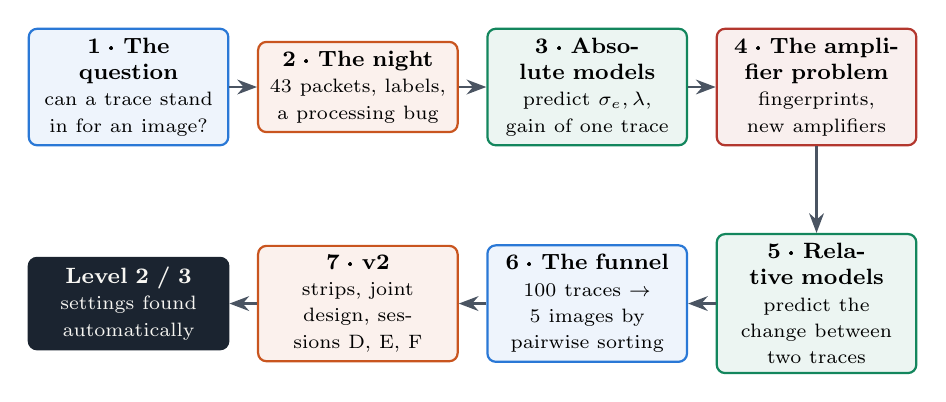
\begin{tikzpicture}[node distance=0.35cm]
\node[box=trace,text width=2.3cm,hl on=<1>] (a) {\textbf{1 \textperiodcentered{} The question}\\\scriptsize can a trace stand in for an image?};
\node[box=image,right=of a,text width=2.3cm,hl on=<2>] (b) {\textbf{2 \textperiodcentered{} The night}\\\scriptsize 43 packets, labels, a processing bug};
\node[box=model,right=of b,text width=2.3cm,hl on=<3>] (c) {\textbf{3 \textperiodcentered{} Absolute models}\\\scriptsize predict $\sigma_e,\lambda$, gain of one trace};
\node[box=problem,right=of c,text width=2.3cm,hl on=<4>] (d) {\textbf{4 \textperiodcentered{} The amplifier problem}\\\scriptsize fingerprints, new amplifiers};
\node[box=model,below=1.1cm of d,text width=2.3cm,hl on=<5>] (e) {\textbf{5 \textperiodcentered{} Relative models}\\\scriptsize predict the change between two traces};
\node[box=trace,left=of e,text width=2.3cm,hl on=<6>] (f) {\textbf{6 \textperiodcentered{} The funnel}\\\scriptsize 100 traces $\to$ 5 images by pairwise sorting};
\node[box=image,left=of f,text width=2.3cm,hl on=<7>] (g) {\textbf{7 \textperiodcentered{} v2}\\\scriptsize strips, joint design, sessions D, E, F};
\node[box=ink,left=of g,text width=2.3cm,fill=ink,text=paper] (h) {\textbf{Level 2 / 3}\\\scriptsize settings found automatically};
\draw[arr] (a)--(b); \draw[arr] (b)--(c); \draw[arr] (c)--(d); \draw[arr] (d)--(e); \draw[arr] (e)--(f); \draw[arr] (f)--(g); \draw[arr] (g)--(h);
\end{tikzpicture}}
\end{center}
\vspace{0.4em}
\begin{columns}[T]
\column{0.32\textwidth}\scriptsize\textbf{Read it as a chain of reasons.} Each step ends with a conclusion, and that conclusion is why the next step exists.
\column{0.32\textwidth}\scriptsize\textbf{Every model is mentioned.} The figures focus on the best ones and the most instructive failures.
\column{0.32\textwidth}\scriptsize\textbf{Captions.} Every figure says \textcolor{trace}{\bfseries what you see} and \textcolor{model}{\bfseries what it means}.
\end{columns}
\end{frame}

% ============================================================================================================
\divider{Step 1}{The question: can a two-second trace stand in for a ten-minute image?}{trace!60}
\section{1 The question}

\begin{frame}{Tuning a CCD means trying settings, and every try costs an image}
\eyebrow{The goal}
\begin{columns}[T]
\column{0.32\textwidth}
{\color{image}\bfseries IMAGE}\par{\Large\bfseries $\sim$5--10 min}\par\small 16 rows $\times$ 1000 columns $\times$ 500 skips. run\_WADERs fits it and gives the truth: $\sigma_e$, $\lambda$, gain.
\column{0.32\textwidth}
{\color{trace}\bfseries TRACE}\par{\Large\bfseries $\sim$2 s}\par\small $2\times5$ pixels $\times$ 500 skips, every raw ADC sample kept.
\column{0.32\textwidth}
{\color{model}\bfseries LEVEL-1 QUESTION}\par\normalsize\bfseries Does the trace already tell us what the image will show?\par\mdseries\small If yes: scan settings with traces, image only the best.
\end{columns}
\vspace{1em}
\begin{columns}[T]
\column{0.32\textwidth}\small {\color{image}\bfseries $\sigma_e$} read noise (e$^-$): width of the 0-electron peak; 0.15--0.19 here.
\column{0.32\textwidth}\small {\color{image}\bfseries $\lambda$} dark charge (e$^-$/pixel): dark current while rows wait + clock-induced charge.
\column{0.32\textwidth}\small {\color{image}\bfseries $g$} gain (ADU/e$^-$): spacing of the electron peaks; 1.26--1.34.
\end{columns}
\vspace{0.8em}
\[
\sigma_{\rm ADU}^2(N)=\frac{\sigma_1^2}{N}+\sigma_{\rm floor}^2,\qquad \sigma_e=\frac{\sigma_{\rm ADU}}{g}\qquad(\sigma_1\approx5.6\ \mathrm{ADU},\ N=500\ \text{skips})
\]
\end{frame}

\begin{frame}{A trace is the raw waveform of 10 pixels, every ADC sample kept}
\eyebrow{The input}
\figright{0.74}{reuse_t_trace_anatomy}
{The raw ADC samples of one pixel's skips. Each skip has a \textbf{pedestal window} (before the charge is dumped onto the sense node), the \textbf{charge transfer}, and a \textbf{signal window}. The vertical structure is the reset pulse and the summing-well dip.}
{CDS (signal $-$ pedestal) gives one number per skip, 500 per pixel. The image keeps only the pixel \emph{averages}. The trace keeps the whole waveform, so it can show \emph{why} the noise is what it is: ringing, slow drifts, pickup, the shape of the edges.}
\end{frame}

\begin{frame}{Every trace becomes 141 numbers and 16 curves}
\eyebrow{From a trace to model inputs}
\figright{0.66}{reuse_t_trace_noise}
{Noise measured from the trace: the Allan deviation of the CDS values against the number of skips averaged, fitted as $\sigma_A^2(n)=a^2/n+b^2$, with $a$ = white noise per skip and $b$ = the slow-noise floor.}
{The 141 scalar features (src/trace\_features.py) cover noise, skip structure, edges, slow drifts and clock pickup. The 16 curves (Allan, spectra, mean skip shape, start transient) feed the networks. \textbf{Feature tiers} (A1 38, A2 38, B 19, C 46, protected P 8) were fixed from the traces alone, \emph{before any label was looked at}, so the feature choice cannot be tuned to the answer.}
\end{frame}

\begin{frame}{A packet: reference traces, one change, new traces, one image}
\eyebrow{The unit of data (v1)}
\begin{center}
\resizebox{\textwidth}{!}{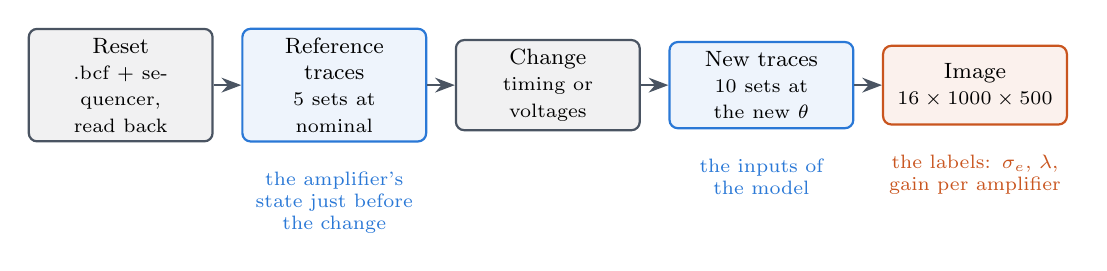
\begin{tikzpicture}[node distance=0.35cm]
\node[box,visible on=<1->] (a) {Reset\\\scriptsize .bcf + sequencer, read back};
\node[box=trace,right=of a,visible on=<2->] (b) {Reference traces\\\scriptsize 5 sets at nominal};
\node[box,right=of b,visible on=<3->] (c) {Change\\\scriptsize timing or voltages};
\node[box=trace,right=of c,visible on=<4->] (d) {New traces\\\scriptsize 10 sets at the new $\theta$};
\node[box=image,right=of d,visible on=<5->] (e) {Image\\\scriptsize $16\times1000\times500$};
\draw[arr,visible on=<2->] (a)--(b); \draw[arr,visible on=<3->] (b)--(c); \draw[arr,visible on=<4->] (c)--(d); \draw[arr,visible on=<5->] (d)--(e);
\node[below=0.25cm of b,font=\scriptsize,text width=2.4cm,align=center,color=trace,visible on=<2->] {the amplifier's state just before the change};
\node[below=0.25cm of d,font=\scriptsize,text width=2.4cm,align=center,color=trace,visible on=<4->] {the inputs of the model};
\node[below=0.25cm of e,font=\scriptsize,text width=2.4cm,align=center,color=image,visible on=<5->] {the labels: $\sigma_e$, $\lambda$, gain per amplifier};
\end{tikzpicture}}
\end{center}
\vspace{0.6em}
\begin{columns}[T]
\column{0.32\textwidth}\small\textbf{Session A} (17 packets)\par\scriptsize timing knobs, one at a time: delayInt, delay\_H, delayRGH \ldots
\column{0.32\textwidth}\small\textbf{Session B} (15 packets)\par\scriptsize voltages, one at a time: VDD, VR, RG, SW, clock rails, VSUB
\column{0.32\textwidth}\small\textbf{Session C} (11 packets)\par\scriptsize many knobs at once, \textbf{sealed}: the honest test, opened once
\end{columns}
\takeaway{one packet = one setting $\theta$ = one image (the truth) plus traces before and after the change. Four amplifiers (ch0--ch3) are read at once, so each packet gives four rows.}
\end{frame}

\begin{frame}{From raw files to a training table}
\eyebrow{Processing}
\begin{center}
\resizebox{!}{0.36\textheight}{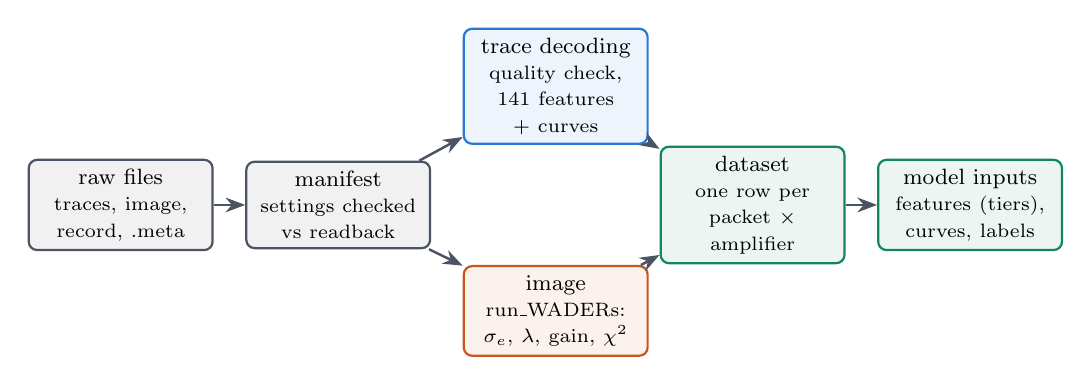
\begin{tikzpicture}[node distance=0.4cm]
\node[box,visible on=<1->] (r) {raw files\\\scriptsize traces, image, record, .meta};
\node[box,right=of r,visible on=<2->] (m) {manifest\\\scriptsize settings checked vs readback};
\node[box=trace,above right=0.2cm and 0.4cm of m,visible on=<3->] (t) {trace decoding\\\scriptsize quality check, 141 features + curves};
\node[box=image,below right=0.2cm and 0.4cm of m,visible on=<4->] (i) {image\\\scriptsize run\_WADERs: $\sigma_e$, $\lambda$, gain, $\chi^2$};
\node[box=model,right=2.9cm of m,visible on=<5->] (d) {dataset\\\scriptsize one row per packet $\times$ amplifier};
\node[box=model,right=of d,visible on=<6->] (x) {model inputs\\\scriptsize features (tiers), curves, labels};
\draw[arr,visible on=<2->] (r)--(m); \draw[arr,visible on=<3->] (m)--(t); \draw[arr,visible on=<4->] (m)--(i);
\draw[arr,visible on=<5->] (t)--(d); \draw[arr,visible on=<5->] (i)--(d); \draw[arr,visible on=<6->] (d)--(x);
\end{tikzpicture}}
\end{center}
\vspace{0.5em}
\begin{columns}[T]
\column{0.48\textwidth}\scriptsize
\textbf{Checks on the way.} Every requested setting must arrive in the readback (VSUB reads 0.2--0.25 V high: the potentiometer step). Damaged traces (no complete CDS window, unequal skip counts) are marked unusable instead of crashing. An image whose WADERs fit has $\chi^2/\mathrm{ndf}>3$ is flagged and left out of training.
\column{0.48\textwidth}\scriptsize
\textbf{Labels are logs.} The targets are $y=(\log\sigma_e,\log\lambda,\log g)$, so errors are relative:
\[\mathrm{error}=100\sqrt{\tfrac1n\textstyle\sum_i(\hat y_i-y_i)^2}\ \%\]
10\,\% means ``typically off by a factor 1.1''.
\end{columns}
\end{frame}

% ============================================================================================================
\divider{Step 2}{The first night: what the data look like, and how good the labels are}{image!70}
\section{2 The night}

\begin{frame}{The night of 2026-11-02 in numbers}
\eyebrow[image]{The data}
\begin{columns}[T]
\column{0.24\textwidth}{\Huge\bfseries 43}\par\small packets, every one at the requested settings
\column{0.24\textwidth}{\Huge\bfseries\color{trace} 92\,\%}\par\small of the board-101 traces usable (2370 of 2580)
\column{0.24\textwidth}{\Huge\bfseries\color{image} 127}\par\small of 128 A+B labels usable after the relabel
\column{0.24\textwidth}{\Huge\bfseries\color{problem} 3}\par\small session-C packets lost every trace at their settings
\end{columns}
\vspace{1.2em}
\begin{columns}[T]
\column{0.48\textwidth}\small\textbf{Training: sessions A + B}\par\scriptsize 32 packets, one knob at a time, 127 rows (4 amplifiers). Setting-grouped cross-validation: a setting's packets are always held out together.
\column{0.48\textwidth}\small\textbf{Test: session C}\par\scriptsize 8 usable packets, knobs changed together, 32 rows. Not looked at until the model choice was frozen (commit 25384b9).
\end{columns}
\vspace{0.8em}
\warnbox{\textbf{Board 102} was read too, but its settings never changed (only acm101 was varied), ch0 and ch1 are dead and its labels scatter 9--13\,\% at nominal. It is used only once, as a ``new module'' test (step 4).}
\end{frame}

\begin{frame}{Twelve hours of packets: settings move the labels, and so does time}
\eyebrow[image]{The night, packet by packet}
\figtop{0.47}{w_night_timeline}
{Each marker is one packet on one amplifier (circle ch0, square ch1, triangle ch3), coloured by the kind of knob changed. Black = nominal packets, joined by grey lines per amplifier. Shaded bands = the 5 contiguous \textbf{time blocks} used as folds in the scorecard (step 5).}
{\textbf{$\lambda$ (top, log scale)} moves by up to $\times4$ with settings, but the nominal packets also drift down $\sim$20\,\% over the night: the CCD's history matters. The outlier near hour 7 is L1\_18, whose queue stalled 38 min with no flush. \textbf{$\sigma_e$ (bottom)} is flat at nominal and rises with timing changes (session A); voltages barely move it. Each amplifier keeps its own level all night.}
\end{frame}

\begin{frame}{How good are the labels? Compare the noise with the effects}
\eyebrow[image]{Label noise}
\figright{0.62}{w_label_noise}
{For each target: grey, the scatter of the nominal packets repeated hours apart; red, the label noise of a \emph{change} (nominal vs nominal); blue, the median true change made by one knob; green, the RMS change within a packet (log scale).}
{$\sigma_e$ is measured well: a typical change (3.9\,\%) is twice its noise. For $\lambda$ the noise (12\,\%) is \emph{larger} than the median one-knob change (8.5\,\%), and the gain changes (0.4\,\%) sit below their noise (0.8\,\%). Many $\lambda$ and gain changes cannot be told from zero, so any score must count only \textbf{clear changes} (larger than the noise).}
\end{frame}

\begin{frame}{A processing bug found by the replicates: the drift correction}
\eyebrow[problem]{Labels first, models second}
\figright{0.6}{w_drift_bug}
{$\sigma_e$ of four packets per amplifier, from run\_WADERs on the raw image (blue) and on the image after our row-start drift correction (red). L1\_06 and L1\_23 have the same setting (delayInt 3000).}
{The correction tripled $\sigma_e$ in places (L1\_03 ch0: 0.24 $\to$ 0.69) and made the replicates disagree by 60\,\% while their traces agreed. This night's images have little drift (raw $\chi^2/\mathrm{ndf}$ 0.8--1.3), so the correction only added noise. It was switched off and all 43 packets relabelled; every result from here on uses the clean labels.}
\takeaway{a model can only be as good as its labels. Replicate packets (same setting, different time) are the cheapest check, and v2 adds them at non-nominal settings too.}
\end{frame}

\begin{frame}{Dark charge remembers the CCD's history}
\eyebrow[problem]{Why $\lambda$ is hard}
\figright{0.62}{fd_fig5_lambda_night}
{$\lambda$ of every packet against the time of night, per amplifier; nominal packets highlighted.}
{At fixed nominal settings $\lambda$ fell about 20\,\% over the night, and one stalled packet (L1\_18, 38 minutes without a flush) came out $\times4$ too high. $\lambda$ depends on the CCD's state as well as on the settings. Later we found its unpredictable part sits in the array (time since the last flush), not in the serial register. v2 therefore flushes right before every image and repeats nominal every 7 packets to track the drift.}
\end{frame}

% ============================================================================================================
\divider{Step 3}{Absolute models: predict the image's $\sigma_e$, $\lambda$ and gain from one trace}{model!60}
\section{3 Absolute models}

\begin{frame}{Seventeen models in four families: the ones that matter are highlighted}
\eyebrow[model]{The model zoo}
\small
\begin{tabular}{p{2.6cm}p{5.3cm}p{5.3cm}}\toprule
family & models & idea\\\midrule
\textbf{baselines} & mean, amplifier mean, \textbf{settings GP}, \textbf{settings + amplifier GP / trees} & no trace at all: what the knobs and the amplifier's identity alone predict\\
\textbf{physics-structured} & physics, \textcolor{model}{\textbf{physics\_white}}, physics\_joint, physics\_hier, sets, physics\_cnn & measure what the trace can measure ($w^2/N$), learn only the rest\\
\textbf{flexible} & ridge, gp, \textcolor{model}{\textbf{gp\_dim}}, gp\_saas, \textcolor{model}{\textbf{boosted trees}}, nn & map features $\to$ labels with no physics\\
\textbf{curve networks} & cnn, \textcolor{model}{\textbf{pretrained cnn}}, deep kernel & learn features from the 16 curves\\\bottomrule
\end{tabular}
\vspace{0.8em}
\begin{columns}[T]
\column{0.48\textwidth}\scriptsize
\textbf{physics\_white}, the star of $\sigma_e$:
\[\log\hat\sigma_e=\tfrac12\log\frac{w^2}{N}-\log\hat g(x)+\hat r(x)\]
$w$ = the trace's white noise per skip (measured), $\hat g$ = learned gain, $\hat r$ = small learned correction (a GP).
\column{0.48\textwidth}\scriptsize
\textbf{Why ``white''.} The first physics model used the Allan floor extrapolated to $n=500$. On real traces that floor jumps between packets ($\times1.45$ vs $\times1.17$ at the same setting), which nothing can learn. Using the white noise instead cut its CV error from 30.6 to 12.6\,\%.
\end{columns}
\end{frame}

\begin{frame}{The protocol: choose on A+B, freeze, then open session C once}
\eyebrow[model]{Honest testing}
\figright{0.6}{reuse_m_cv}
{Setting-grouped cross-validation on A+B: all packets of one setting (e.g.\ the four nominal ones) are held out together, so a model is never tested on a setting it trained on.}
{(1) label-free feature tiers, frozen; (2) every model at every feature set, scored by CV on A+B; (3) the choice written down and committed: $\sigma_e$ gp\_dim, $\lambda$ pretrained cnn, gain gp\_dim; (4) only then session C scored, once. This guards against fooling ourselves, and it caught exactly that (next slides).}
\end{frame}

\begin{frame}{Cross-validation on A+B: trace models beat the settings for every target}
\eyebrow[model]{Training data}
\figright{0.66}{w_cv_models}
{Error (\%) of every model on the A+B cross-validation (clean labels), grey = no trace, green = physics family, blue = flexible and network models. Dashed: settings-only. Outlined: the best per target. Ridge (103\,\%, unstable) is left out.}
{The traces help: $\sigma_e$ 17.9 $\to$ 11.8\,\% (pretrained cnn), $\lambda$ 46 $\to$ 29\,\% (trees), gain 2.7 $\to$ 0.8\,\% (trees). The Allan-floor physics model (30.6\,\%) is the one failure, fixed by physics\_white. On the feature ladder gp\_dim reached 10.5\,\% on $\sigma_e$ and was frozen as the choice.}
\end{frame}

\begin{frame}{Session C, opened once: the physics model wins, the frozen choice does not}
\eyebrow[model]{The prospective test}
\figtop{0.46}{fd_fig1_traces_help}
{Typical error per target, on the A+B cross-validation (left group) and on the sealed session C (right group). Grey: always the average. Light blue: settings + which amplifier, no trace. Blue: the frozen trace model (chosen on A+B). Orange: the physics-structured model. Dashed: label noise.}
{\textbf{$\lambda$: 5.3\,\%} (physics) vs 23.2\,\% without a trace, significant. \textbf{$\sigma_e$: 7.3\,\%} (physics\_white) vs 10.2\,\%, not significant with 8 packets. \textbf{Gain: 0.9\,\%} vs 1.4\,\%. The frozen flexible choice failed $\sigma_e$ (gp\_dim 13.5\,\%, worse than no trace).}
\end{frame}

\begin{frame}{Why cross-validation ranked the models wrong}
\eyebrow[problem]{Extrapolation vs interpolation}
\figright{0.74}{fd_fig7_all_models}
{Every model: open circle = A+B cross-validation, filled = session C, per target.}
{Flexible models (gp\_dim, trees, nn) looked best in CV and fell back on C; physics-structured ones did the opposite. A+B changed one knob at a time, so holding out a setting asks the model to \emph{extrapolate} along a knob it never saw move. C moves all knobs inside the range, which is \emph{interpolation}. The lesson for v2: a \textbf{joint design}, so training and test ask the same kind of question.}
\end{frame}

\begin{frame}{Session C, amplifier by amplifier}
\eyebrow[model]{Predicted vs true}
\figright{0.76}{fd_fig2_session_c}
{Predicted vs true label for each session-C row, per target. Top row: the frozen choice. Bottom row: the physics-structured models. Band: $\pm$ the label scatter. Grey dots: the A+B training rows.}
{$\lambda$ follows the diagonal across a factor of 3 with the physics model. $\sigma_e$ is tight for physics\_white but scatters for the frozen gp\_dim. The gain is a narrow range (1.26--1.34) where every model mostly predicts the amplifier's own level.}
\end{frame}

\begin{frame}{Where $\sigma_e$ goes wrong: timing changes the image more than the trace}
\eyebrow[problem]{A physics gap}
\figright{0.76}{fd_fig4_trace_vs_image}
{Image $\sigma_e$ against the trace's white noise per skip, one point per packet $\times$ amplifier; voltage packets (session B) and timing packets (session A).}
{Voltage packets sit on one line: the trace's noise predicts the image's. Timing packets scatter off it (delay\_Ha 3600 raises image $\sigma_e$ 45\,\% with no change in the trace). The trace reads 10 pixels after a 100-column burst; the image reads $10^4$ pixels after a 5300-column prescan and a clear. Session A is 43\,\% of the rows but \textbf{76\,\%} of the squared error. A level-1 \emph{strip} read exactly like the image closes this gap (step 7).}
\end{frame}

\begin{frame}{What each model relies on: shuffle one input group at a time}
\eyebrow[model]{Explaining the models}
\figright{0.74}{fd_fig8_reliance}
{Heat map: how far each model's prediction moves when one group of inputs is shuffled ($S_G$), and how much its session-C error rises ($L_G$). Also shuffled \emph{within} each amplifier.}
{Gain comes from recognising the amplifier: shuffling the reference-trace noise features moves it 3.5\,\%, but only 0.5\,\% within an amplifier. $\lambda$ uses amplifier recognition (C loss 46 points) \emph{and} the own trace (18 points, also within an amplifier). $\sigma_e$ (physics\_white) rests on the measured white noise; the flexible models lean on timing proxies, which do not transfer to C.}
\end{frame}

\begin{frame}{Most of the $\sigma_e$ accuracy comes from the measured noise itself}
\eyebrow[model]{Inside physics\_white}
\figtop{0.46}{fd_fig9_physics_terms}
{The session-C $\sigma_e$ error built up term by term: the measured trace term $w/\sqrt N$ with the average gain, then with the learned gain, then with the learned correction.}
{8.8\,\% from the measured white noise alone, 7.6\,\% with the learned gain, 7.3\,\% with the correction (the image is about $0.82\times$ the trace on board 101). The model is mostly a \emph{measurement} with small learned corrections, which is why it generalises.}
\end{frame}

\begin{frame}{Which features help? The feature ladder}
\eyebrow[model]{Feature sets}
\figright{0.7}{fd_fig6_ladder}
{CV error of each model as the feature set grows (none $\to$ P $\to$ P+A1 $\to$ P+A $\to$ P+A+B $\to$ all), per target.}
{With 32 packets the intervals are wide: differences of 1--3 points are not significant. Patterns match the synthetic study: plain gp gains nothing beyond P, gp\_dim takes many features without collapsing, the networks improve up to all features, ridge breaks with trace features. The physics model with the Allan floor stays at 30--35\,\% for every set: its trace term was the problem, not the features.}
\end{frame}

% ============================================================================================================
\divider{Step 4}{The amplifier problem: is the trace predicting the noise, or recognising the amplifier?}{problem!70}
\section{4 The amplifier problem}

\begin{frame}{A sharper baseline: settings plus the amplifier's name}
\eyebrow[problem]{The right question}
\begin{columns}[T]
\column{0.5\textwidth}\small
Each amplifier has its own level of $\sigma_e$, $\lambda$ and gain (step 2). A model that only works out \emph{which amplifier} it is looking at already predicts a lot.\par\medskip
So the fair reference is a model with the settings \textbf{and the amplifier one-hot}, but no trace: \textbf{settings + amplifier} (GP or trees).
\column{0.46\textwidth}\small
{\footnotesize\begin{tabular}{lccc}\toprule
A+B CV, \% & $\sigma_e$ & $\lambda$ & gain\\\midrule
settings + amp, trees & 15.7 & 36.1 & \textbf{0.8}\\
best trace model & \textbf{10.5} & \textbf{27.0} & \textbf{0.8}\\
difference & $-5$ * & $-9$ * & 0\\\bottomrule
\end{tabular}}\par\smallskip
\scriptsize * = 95\,\% packet-bootstrap interval excludes 0
\end{columns}
\vspace{1em}
\begin{columns}[T]
\column{0.32\textwidth}\scriptsize\textbf{Gain:} the traces add nothing beyond the amplifier's name. They act as a fingerprint.
\column{0.32\textwidth}\scriptsize\textbf{$\sigma_e$:} a modest, real gain from the traces.
\column{0.32\textwidth}\scriptsize\textbf{$\lambda$:} the traces clearly help (7--15 points).
\end{columns}
\end{frame}

\begin{frame}{Finding the amplifier fingerprints}
\eyebrow[problem]{Amplifier-identifying features}
\figtop{0.40}{fig_fingerprint}
{Left: the strongest fingerprints. Each bar is how often \emph{one feature alone} names the amplifier of a held-out packet (chance = 0.25). Right: histogram of $\eta^2$, the share of a feature's variance that is just ``which amplifier'', for own-trace (blue) and reference-trace (orange) features.}
{\[\eta^2=1-\frac{\sum_a\sum_{i\in a}(x_i-\bar x_a)^2}{\sum_i(x_i-\bar x)^2}\]
Reference-trace features (always at nominal) are almost all fingerprints: edge ringing, dip depth, within-cycle power. \textbf{52 columns} have $\eta^2>0.9$ (46 reference, 6 own). Own-trace noise features are not: white noise $\eta^2=0.09$.}
\end{frame}

\begin{frame}{On an amplifier the model never saw, the levels are lost}
\eyebrow[problem]{Leave one amplifier out}
\figtop{0.44}{fig_loao}
{Error on each amplifier when trained on the other three (4 amplifiers $\times$ 5 packet folds), per model and target; light bars after removing the amplifier's mean offset (``shape'' only).}
{\textbf{$\sigma_e$:} physics\_white 12.3 $\to$ 14.0\,\% on a new amplifier; the flexible models fall back to the average (18.7\,\%). \textbf{$\lambda$ and gain:} no model beats the mean's level (55\,\%, 3.5\,\%). Once the offset is removed, $\lambda$'s shape is learnt (physics 28 vs 37\,\%). \textbf{The level does not transfer; the shape does.}}
\end{frame}

\begin{frame}{Remove the fingerprints: $\lambda$ and gain suffer, $\sigma_e$ does not care}
\eyebrow[problem]{Ablation}
\figtop{0.44}{fig_no_fingerprint}
{Session-C and new-amplifier errors with all features, without the $\eta^2>0.9$ columns (eta90, 52 removed), and without $\eta^2>0.5$ (eta50, 93 removed).}
{\textbf{$\lambda$:} physics 5.3 $\to$ 15.2\,\%, still better than settings + amplifier (23\,\%), so part of $\lambda$ is real trace information. \textbf{Gain:} physics 0.9 $\to$ 2.8\,\%: it came from recognising the amplifier. \textbf{$\sigma_e$:} 7.3 $\to$ 6.9\,\%: it never used them. On new amplifiers the curve models gain a little (cnn $\lambda$ 64 $\to$ 52\,\%).}
\end{frame}

\begin{frame}{Why recognising the amplifier is not predicting its gain}
\eyebrow[problem]{The physics behind it}
\begin{columns}[T]
\column{0.5\textwidth}\small
\textbf{On known amplifiers} the model learns a lookup: ``ringing rms $\approx$ 12 ADU $\to$ ch0 $\to$ gain 1.34''.\par\medskip
\textbf{On a new amplifier} the fingerprint value has no gain attached, and three training amplifiers are three points: any curve fits them.
\column{0.46\textwidth}\small
\textbf{The trace is in ADU and holds no known charge:}
\[\sigma_1^{\rm ADU}=\sigma_e\times g\]
A quiet, high-gain amplifier looks just like a noisy, low-gain one. Only whole electrons (the image's peaks, or a strip's) separate them.
\end{columns}
\vspace{1em}
\begin{center}
\resizebox{!}{0.26\textheight}{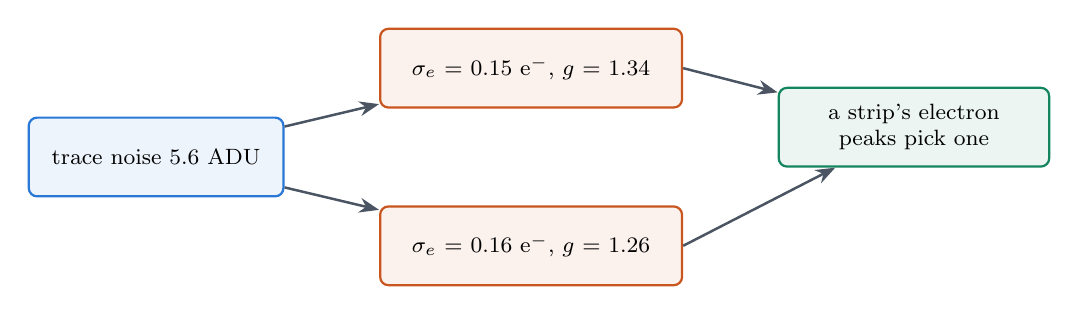
\begin{tikzpicture}[node distance=0.5cm]
\node[box=trace,text width=3cm,visible on=<1->] (a) {trace noise 5.6 ADU};
\node[box=image,above right=0.1cm and 1.2cm of a,text width=3.6cm,visible on=<2->] (b) {$\sigma_e$ = 0.15 e$^-$, $g$ = 1.34};
\node[box=image,below right=0.1cm and 1.2cm of a,text width=3.6cm,visible on=<2->] (c) {$\sigma_e$ = 0.16 e$^-$, $g$ = 1.26};
\node[box=model,right=1.2cm of b,text width=3.2cm,visible on=<3->,yshift=-0.75cm] (d) {a strip's electron peaks pick one};
\draw[arr,visible on=<2->] (a)--(b); \draw[arr,visible on=<2->] (a)--(c);
\draw[arr,visible on=<3->] (b.east)--(d); \draw[arr,visible on=<3->] (c.east)--(d);
\end{tikzpicture}}
\end{center}
\end{frame}

\begin{frame}{Another module: trained on board 101, tested on board 102}
\eyebrow[problem]{A second board}
\figright{0.56}{fig_board102}
{Predictions for board-102 ch2 (41 rows, all at nominal) by models trained on board 101, before and after subtracting the first image's offset.}
{The levels miss: physics $\sigma_e$ is 30\,\% low (image/trace ratio 1.06 on 102 vs 0.82 on 101), and $\lambda$ is 1.11 e$^-$/pixel, 2--4$\times$ board 101. \textbf{After one image}, every model sits at the label scatter ($\sigma_e$ $\sim$11\,\%, $\lambda$ $\sim$8\,\%, gain 0.3\,\%). One calibration measurement per amplifier is enough to fix the level. A weak test: 102's settings never changed.}
\end{frame}

\begin{frame}{The odd amplifier: dropping 101 ch2 (EXT3)}
\eyebrow[problem]{Data quality per amplifier}
\figright{0.74}{fig_no_ch2}
{Errors scored on ch0, ch1, ch3 only, trained with all four amplifiers, without ch2, and without ch2 and the fingerprints.}
{ch2's per-row $\lambda$ fit has $\chi^2$ 22 (others 3--4) and its $\lambda$ is 0.61 (others 0.27--0.48). Without it, $\lambda$ on a new amplifier improves (physics 70 $\to$ 49 $\to$ 46\,\%, nn 55 $\to$ 47 $\to$ 40\,\%), below the mean (52\,\%) for the first time. ch2 is kept out of the \emph{absolute} models. Step 5 shows it is still useful for the \emph{relative} models.}
\end{frame}

\begin{frame}{Without the settings as input, nothing gets worse}
\eyebrow[model]{Traces only}
\small Every model trained without 101 ch2, without the fingerprints, and \textbf{with} vs \textbf{without} the 67 settings $\theta$ as input. Errors in \%, scored on ch0, ch1, ch3.\par\medskip
\begin{tabular}{lcccc}\toprule
 & \multicolumn{2}{c}{session C} & \multicolumn{2}{c}{new amplifier}\\
model, target & with $\theta$ & without $\theta$ & with $\theta$ & without $\theta$\\\midrule
physics, $\sigma_e$ & 5.9 & 6.1 & 14.4 & 14.9\\
cnn, $\sigma_e$ & 10.0 & 7.0 & 23.4 & 22.5\\
pretrained, $\sigma_e$ & 15.7 & \textbf{5.2} & 17.8 & 19.0\\
physics, $\lambda$ & 10.4 & 10.4 & 46.3 & 46.0\\
cnn, $\lambda$ & 13.2 & 11.8 & 44.4 & \textbf{39.7}\\
deep\_kernel, $\lambda$ & 20.3 & 17.5 & 53.2 & \textbf{42.0}\\
physics, gain & 2.0 & \textbf{0.7} & 3.6 & 3.7\\\bottomrule
\end{tabular}\par\medskip
The trace already carries what the models used the settings for. Traces-only models are simpler and do not learn a map of this CCD's knobs that would not carry to another CCD.
\end{frame}


\begin{frame}{More packets still help}
\eyebrow[model]{Learning curve}
\figtop{0.48}{fig_learning_curve}
{Session-C error when trained on random subsets of 8, 16, 24, 32 A+B packets (5 draws per size), without ch2 and the fingerprints.}
{physics\_white $\sigma_e$ 9.7 $\to$ 5.9\,\% and $\lambda$ 19.0 $\to$ 10.4\,\% from 8 to 32 packets, with no sign of levelling off; cnn $\lambda$ 22.6 $\to$ 12.7\,\%. Gain flattens near 1\,\% (the label noise). \textbf{More data is the cheapest improvement left}: v2 has 61 training packets plus 15 held out.}
\end{frame}

\begin{frame}{Conclusion of steps 3--4: learn the shape, measure the level}
\eyebrow[model]{What carries to another amplifier}
\[\log y(\theta,a)=c_a+f(\theta,\mathrm{trace}),\qquad c_a=\log y_{\rm measured}(\theta_0)-f(\theta_0)\]
\begin{columns}[T]
\column{0.32\textwidth}{\color{model}\bfseries $f$: learned}\par\small how the value moves with settings and the CCD's state; carries over (LOAO shape, board 102 after one image)
\column{0.32\textwidth}{\color{image}\bfseries $c_a$: measured}\par\small one number per amplifier and target, from one image or a strip; cannot be learned from a trace (gain $\times\sigma_e$ degeneracy)
\column{0.32\textwidth}{\color{trace}\bfseries how often}\par\small gain and $\sigma_e$ factor are stable (0.6\,\%, 2\,\%); $\lambda$ drifts 20\,\% a night
\end{columns}
\vspace{1em}
\begin{center}
\resizebox{0.9\textwidth}{!}{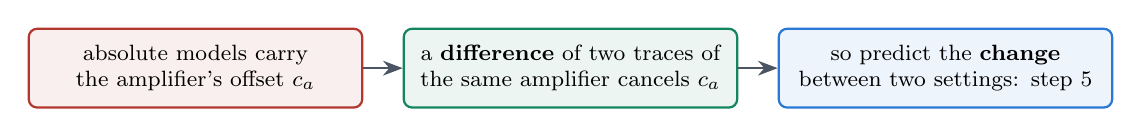
\begin{tikzpicture}[node distance=0.5cm]
\node[box=problem,text width=4cm,visible on=<1->] (a) {absolute models carry the amplifier's offset $c_a$};
\node[box=model,right=of a,text width=4cm,visible on=<2->] (b) {a \textbf{difference} of two traces of the same amplifier cancels $c_a$};
\node[box=trace,right=of b,text width=4cm,visible on=<3->] (c) {so predict the \textbf{change} between two settings: step 5};
\draw[arr,visible on=<2->] (a)--(b); \draw[arr,visible on=<3->] (b)--(c);
\end{tikzpicture}}
\end{center}
\end{frame}

% ============================================================================================================
\divider{Step 5}{Relative models: predict the change between two traces}{model!60}
\section{5 Relative models}

\begin{frame}{The idea: compare two traces of the same amplifier}
\eyebrow[model]{Relative (change) models}
\begin{center}
\resizebox{0.95\textwidth}{!}{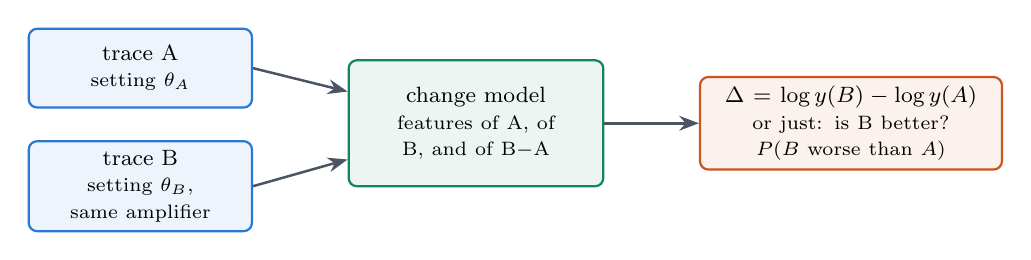
\begin{tikzpicture}[node distance=0.5cm]
\node[box=trace,text width=2.6cm,visible on=<1->] (a) {trace A\\\scriptsize setting $\theta_A$};
\node[box=trace,below=0.4cm of a,text width=2.6cm,visible on=<1->] (b) {trace B\\\scriptsize setting $\theta_B$, same amplifier};
\node[box=model,right=1.2cm of a,yshift=-0.7cm,text width=3cm,minimum height=1.6cm,visible on=<2->] (m) {change model\\\scriptsize features of A, of B, and of B$-$A};
\node[box=image,right=1.2cm of m,text width=3.6cm,visible on=<3->] (o) {$\Delta=\log y(B)-\log y(A)$\\\scriptsize or just: is B better? $P(B\ \text{worse than}\ A)$};
\draw[arr,visible on=<2->] (a.east)--(m); \draw[arr,visible on=<2->] (b.east)--(m); \draw[arr,visible on=<3->] (m)--(o);
\end{tikzpicture}}
\end{center}
\vspace{0.6em}
\begin{columns}[T]
\column{0.48\textwidth}\scriptsize
\textbf{Why it should transfer.} If $\log y=c_a+f(\mathrm{trace})$, then
\[\Delta=f(B)-f(A):\quad c_a\ \text{cancels.}\]
The amplifier's level, the thing that did not carry over, is not needed.
\column{0.48\textwidth}\scriptsize
\textbf{Why it is what level 2 needs.} Optimising settings only asks ``is the candidate better than the incumbent?'' A model that answers that from two traces can steer a search without an image per step.
\end{columns}
\end{frame}

\begin{frame}{What two subtracted traces look like}
\eyebrow[model]{The inputs of a change model}
\figright{0.72}{subtracted_traces_example}
{Top: the raw difference B $-$ A of two traces (L1\_04 delayInt 300, L1\_16 VR). The clock pulses are out of phase, so the raw difference is dominated by edges and the noise is invisible. Below: the \emph{difference curves} the models use, i.e.\ the difference of each trace's Allan curve, spectrum and mean skip shape.}
{Subtracting raw waveforms does not work: a timing change shifts every edge. Subtracting \emph{summaries} of each trace (features and curves) does: they are aligned by construction, and the difference shows where the noise changed (short-window noise, within-cycle spectrum). These are the B$-$A inputs.}
\end{frame}

\begin{frame}{Which parts of the difference curves follow the change of the labels}
\eyebrow[model]{Where the information is}
\figright{0.72}{difference_curve_correlation}
{Correlation, across within-packet changes, between each point of each difference curve and the change of $\sigma_e$ (top) or $\lambda$ (bottom).}
{$\Delta\sigma_e$ tracks the change of the mean skip shape ($|r|$ 0.74), the within-cycle structure function and spectrum, and noise vs window length. $\Delta\lambda$ tracks the within-cycle spectrum (0.60), the CDS spectrum and the CDS autocorrelation. These located the \textbf{hand-picked bands}: 6 bands per target, chosen inside each training fold.}
\end{frame}

\begin{frame}{The change models we built}
\eyebrow[model]{Model variants}
\small
\begin{tabular}{p{4.1cm}p{5.0cm}p{4.0cm}}\toprule
model & inputs & verdict\\\midrule
trees on B$-$A & feature differences & solid baseline\\
\textcolor{model}{\textbf{trees on [A, B, B$-$A]}} & A's and B's features and their difference & \textcolor{model}{\textbf{best on new amplifiers}}\\
trees on [A, B$-$A] & without B & worse on new amps ($\lambda$ size 53\,\%)\\
hand-picked bands + GP & 6 bands of the difference curves + $\Delta w$ & best size on C ($\sigma_e$ 6.6\,\%); adds nothing to trees\\
shared-encoder (Siamese) net & the same encoder for A and B & no better; overfits 84 rows\\
difference of two absolute models & $f(B)-f(A)$ & good direction, no worse size\\
settings-change GP & $\theta_B-\theta_A$, no trace & the reference to beat\\\bottomrule
\end{tabular}
\vspace{0.6em}
\begin{columns}[T]
\column{0.48\textwidth}\scriptsize\textbf{Both orders.} Every training pair is used as (A,B) with label $\Delta$ and as (B,A) with $-\Delta$, so the model is antisymmetric and has no ``up'' bias.
\column{0.48\textwidth}\scriptsize\textbf{Two scores.} \emph{Direction} (right sign on clear changes, i.e.\ larger than the label noise) and \emph{size} (RMS error of $\Delta$).
\end{columns}
\end{frame}

\begin{frame}{The four-way scorecard}
\eyebrow[model]{How every model is rated}
\begin{center}
\resizebox{!}{0.56\textheight}{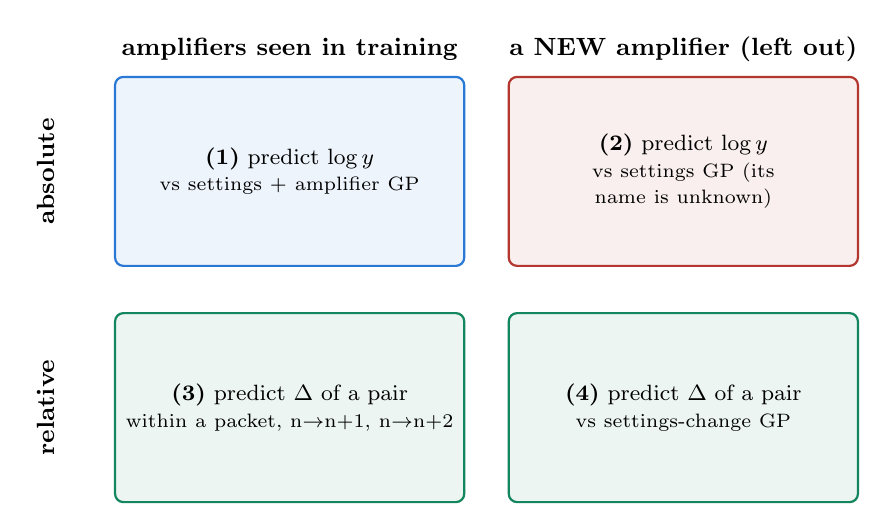
\begin{tikzpicture}
\node[font=\small\bfseries] at (2.5,3.3) {amplifiers seen in training};
\node[font=\small\bfseries] at (7.5,3.3) {a NEW amplifier (left out)};
\node[font=\small\bfseries,rotate=90] at (-0.6,1.75) {absolute};
\node[font=\small\bfseries,rotate=90] at (-0.6,-1.25) {relative};
\node[box=trace,text width=4.2cm,minimum height=2.4cm,visible on=<1->] at (2.5,1.75) {\textbf{(1)} predict $\log y$\\\scriptsize vs settings + amplifier GP};
\node[box=problem,text width=4.2cm,minimum height=2.4cm,visible on=<2->] at (7.5,1.75) {\textbf{(2)} predict $\log y$\\\scriptsize vs settings GP (its name is unknown)};
\node[box=model,text width=4.2cm,minimum height=2.4cm,visible on=<3->] at (2.5,-1.25) {\textbf{(3)} predict $\Delta$ of a pair\\\scriptsize within a packet, n$\to$n+1, n$\to$n+2};
\node[box=model,text width=4.2cm,minimum height=2.4cm,visible on=<4->] at (7.5,-1.25) {\textbf{(4)} predict $\Delta$ of a pair\\\scriptsize vs settings-change GP};
\end{tikzpicture}}
\end{center}
\scriptsize Board 101 ch0/1/3, 40 packets with traces. Folds = 5 contiguous \textbf{time blocks}; ``new amplifier'' = leave one amplifier out \emph{and} a block out. Trace models never see the settings. Every model is compared with its cell's settings-only reference by a packet bootstrap (95\,\%): better / same / worse. Plus \textbf{(5)}: can the predictions rank the settings? (step 6).
\end{frame}

\begin{frame}{Scorecard results: where the traces beat the settings}
\eyebrow[model]{The four cells}
\figright{0.8}{w_scorecard_grid}
{For each cell and target: orange = the settings-only reference, blue = the best trace model (named in the bar), with the bootstrap verdict. Top row: error (log scale, lower is better). Bottom row: direction right on clear n$\to$n+1 changes (higher is better; 50\,\% = coin flip).}
{\textbf{(1)} On known amplifiers, traces win for $\lambda$ (28 vs 37\,\%) and gain. \textbf{(2)} On a new amplifier nothing wins reliably except cnn on $\lambda$ (41 vs 49\,\%). \textbf{(3), (4)} Between packets, trace change models get the direction right 74--89\,\% of the time, ahead of the settings in most cells, but \textbf{not significant}: about 50 clear changes each. More pairs are needed (v2).}
\end{frame}

\begin{frame}{A trap: within a packet, ``always up'' scores 96\,\%}
\eyebrow[problem]{The base rate}
\figtop{0.40}{w_base_rate}
{Hatched bars: the share of clear changes that go \emph{up}, i.e.\ the score of a model that always says ``worse''. Dots: two models' direction scores. Left: within-packet changes (nominal $\to$ new). Right: neighbouring packets (n$\to$n+1).}
{Nominal is near the best setting, so moving away from it almost always makes $\sigma_e$ worse (96\,\%). An earlier ``94\,\% direction'' result was mostly this base rate. Fixes: train on both orders, report the base rate, and judge direction on \textbf{balanced} pairs (neighbours: 50\,\% up). v2 also takes 21 references at the previous packet's settings, not nominal.}
\end{frame}

\begin{frame}{The offset really cancels: ch2 as a new amplifier}
\eyebrow[model]{Does the change model remove the amplifier bias?}
\figright{0.78}{w_ch2_offset}
{Mean error (prediction $-$ truth, \%) on board-101 ch2 when it is the left-out amplifier. Red: absolute models. Blue: change models and differences of absolute models, on n$\to$n+1 pairs. Left $\lambda$, right $\sigma_e$.}
{The absolute models miss ch2's level by $-54$ to $-100$\,\% in $\lambda$ (its odd offset). Every change model is within $-7$ to $+2$\,\%: \textbf{the amplifier's offset cancels in a difference}, as the algebra says. Adding ch2 to training leaves the change models unchanged within their intervals but makes the absolute models worse. \textbf{ch2 is usable as training data for change models only.}}
\end{frame}

\begin{frame}{Which change model? Give it A, B and B$-$A}
\eyebrow[model]{Combined models}
\figtop{0.42}{w_combined_models}
{New amplifier, all between-packet pairs (n+1 and n+2, 231 pairs). Left: direction right on clear changes. Right: size error (log scale). Orange: settings-change GP. Blues: tree models with different inputs; outlined = [A, B, B$-$A].}
{Giving the trees A's and B's own features as well as the difference is best: 75 / 89 / 88\,\% ($\sigma_e$ / $\lambda$ / gain) vs 70 / 88 / 86\,\% for B$-$A alone and 68 / 75 / 73\,\% for the settings (differences n.s.). The model can learn ``this change matters more when A is already noisy''. Hand-picked bands add nothing on top.}
\end{frame}

\begin{frame}{Does it work for every kind of change?}
\eyebrow[model]{Nominal + delayInt vs nominal + VR, and others}
\figright{0.76}{w_kind_heatmap}
{Direction right on clear changes for the combined model on a new amplifier, split by which kinds of knob the two traces differ in. Upper block: nominal vs one kind. Lower block: two changed settings compared directly. Faded = fewer than 5 clear changes.}
{\textbf{Timing works} (nominal vs timing: $\lambda$ 100\,\%, $\sigma_e$ 88\,\%). The output stage moves the gain (89\,\%) but barely $\sigma_e$ or $\lambda$. Clock rails and VSUB gave almost no clear changes in v1. \textbf{Two different kinds} (e.g.\ delayInt vs VR): $\lambda$ 90\,\%, gain 100\,\%, but $\sigma_e$ only 44\,\% of 17 small (5--10\,\%) changes. This comparison is exactly what level 2 needs and v1 has the fewest examples of it.}
\end{frame}

\begin{frame}{Three ways to make training pairs}
\eyebrow[model]{Where the change labels come from}
\begin{center}
\resizebox{!}{0.4\textheight}{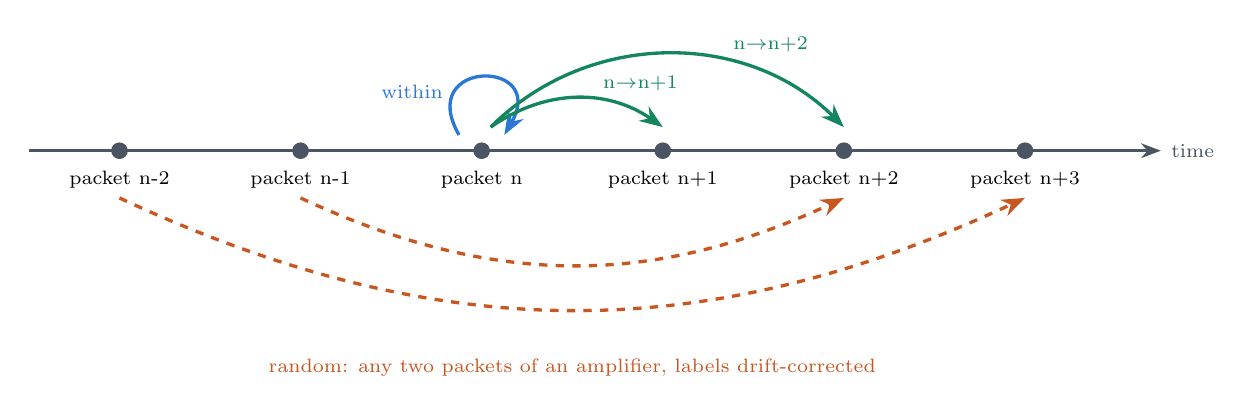
\begin{tikzpicture}[x=1.15cm]
\draw[arr] (0,0)--(12.5,0) node[right,font=\scriptsize] {time};
\foreach \x/\l in {1/n-2,3/n-1,5/n,7/n+1,9/n+2,11/n+3} {\fill[ink2] (\x,0) circle (3pt); \node[below=4pt,font=\scriptsize] at (\x,0) {packet \l};}
\begin{scope}[visible on=<1->]
\draw[trace,line width=1.2pt,-{Stealth}] (4.75,0.2) to[out=120,in=60,looseness=5] node[pos=0.25,left,font=\scriptsize] {within} (5.25,0.2);
\end{scope}
\begin{scope}[visible on=<2->]
\draw[model,line width=1.2pt,-{Stealth}] (5.1,0.3) to[bend left=35] node[pos=0.6,above right=-1pt,font=\scriptsize] {n$\to$n+1} (7,0.3);
\draw[model,line width=1.2pt,-{Stealth}] (5.1,0.3) to[bend left=45] node[pos=0.65,above right=-1pt,font=\scriptsize] {n$\to$n+2} (9,0.3);
\end{scope}
\begin{scope}[visible on=<3->]
\draw[image,line width=1.2pt,-{Stealth},dashed] (1,-0.6) to[bend right=25] (11,-0.6);
\draw[image,line width=1.2pt,-{Stealth},dashed] (3,-0.6) to[bend right=25] (9,-0.6);
\node[image,font=\scriptsize] at (6,-2.75) {random: any two packets of an amplifier, labels drift-corrected};
\end{scope}
\end{tikzpicture}}
\end{center}
\begin{columns}[T]
\column{0.32\textwidth}\scriptsize\textcolor{trace}{\bfseries Within a packet.} Reference (nominal) $\to$ new traces, minutes apart, labels = the image vs the nominal interpolated in time. Few (one per packet) and biased ``up''.
\column{0.32\textwidth}\scriptsize\textcolor{model}{\bfseries Neighbours} $i\pm1$, $i\pm2$. Both images measured 15--30 min apart, raw labels; drift small. Balanced, but only $\sim$4 per packet.
\column{0.32\textwidth}\scriptsize\textcolor{image}{\bfseries Random pairs.} Every two packets: $\binom{n}{2}$ pairs. Label $e(B)-e(A)$ with the \emph{setting effect} $e=\log y-\log y_{\rm nominal}(t)$, drift removed by interpolating the nominal packets.
\end{columns}
\end{frame}

\begin{frame}{The ranking only needs a direction: a classifier that ignores noise-sized changes}
\eyebrow[model]{Direction classifier}
\figright{0.56}{w_direction_weight}
{The weight a training pair gets, against the size of its true change, for each target. Dotted lines: the label noise of a change.}
{Boosted-tree \textbf{classifiers} predict $P(B\ \text{worse than}\ A)$. A pair whose change is smaller than the label noise is a coin flip in the data, so it is down-weighted:
\[w=1-e^{-\Delta^2/2s^2},\quad s=1.9,\ 12,\ 0.8\,\%\]
($\sigma_e$, $\lambda$, gain). The model returns the margin $P-\tfrac12$, which the sorting step uses as a soft win.}
\end{frame}

\begin{frame}{Which pairs and which target? Random pairs and the direction classifier}
\eyebrow[model]{Training choices, tested by ranking}
\figtop{0.42}{w_pairs_target}
{Spearman correlation between the true $\lambda$ order of the 35 first-night settings and the order produced by screen-vs-screen Bradley--Terry sorting (step 6), for size-regression vs direction models, trained on random vs neighbour pairs (hatched).}
{\textbf{Direction + random pairs} ranks best: 0.84 (trained amplifiers) and 0.85 (new amplifier). Random drift-corrected pairs beat neighbours for ranking, even though neighbours are slightly better for single $\lambda$ pairs (90 vs 85\,\%): many more pairs, all settings compared with all. These are the funnel's defaults.}
\end{frame}

% ============================================================================================================
\divider{Step 6}{The funnel: 100 traces in, a shortlist of 5 out}{trace!60}
\section{6 The funnel}

\begin{frame}{The idea: screen many settings with traces, image only the best}
\eyebrow{Level-2 screening}
\begin{center}
\resizebox{0.95\textwidth}{!}{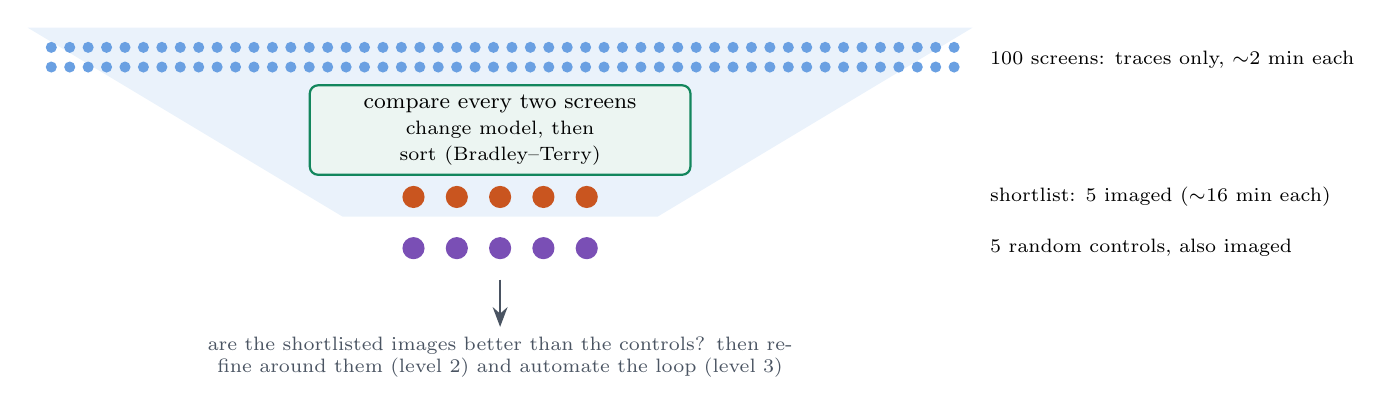
\begin{tikzpicture}
\fill[trace!10,visible on=<1->] (0,3) -- (12,3) -- (8,0.6) -- (4,0.6) -- cycle;
\foreach \i in {0,...,49} {\pgfmathsetmacro{\x}{0.3+0.234*\i} \fill[trace!70,visible on=<1->] (\x,2.75) circle (2pt);}
\foreach \i in {0,...,49} {\pgfmathsetmacro{\x}{0.3+0.234*\i} \fill[trace!70,visible on=<1->] (\x,2.5) circle (2pt);}
\node[font=\scriptsize,right,visible on=<1->] at (12.1,2.6) {100 screens: traces only, $\sim$2 min each};
\node[box=model,text width=4.6cm,visible on=<2->] at (6,1.7) {compare every two screens\\\scriptsize change model, then sort (Bradley--Terry)};
\foreach \i in {0,...,4} {\fill[image,visible on=<3->] (4.9+0.55*\i,0.85) circle (4pt);}
\node[font=\scriptsize,right,visible on=<3->] at (12.1,0.85) {shortlist: 5 imaged ($\sim$16 min each)};
\foreach \i in {0,...,4} {\fill[violet,visible on=<4->] (4.9+0.55*\i,0.2) circle (4pt);}
\node[font=\scriptsize,right,visible on=<4->] at (12.1,0.2) {5 random controls, also imaged};
\draw[arr,visible on=<5->] (6,-0.2) -- (6,-0.8) node[below,font=\scriptsize,text width=9cm,align=center] {are the shortlisted images better than the controls? then refine around them (level 2) and automate the loop (level 3)};
\end{tikzpicture}}
\end{center}
\vspace{0.4em}
\begin{columns}[T]
\column{0.32\textwidth}\scriptsize\textbf{Cost.} 100 images $\approx$ 27 h; 100 trace screens + 10 images $\approx$ 6.9 h.
\column{0.32\textwidth}\scriptsize\textbf{No references.} Each screen is just its new traces: the question is purely ``from 100 traces, which 5 settings are best?''
\column{0.32\textwidth}\scriptsize\textbf{First round: $\lambda$ only.} Rank on dark charge; the predicted $\sigma_e$ is attached to each pick afterwards.
\end{columns}
\end{frame}

\begin{frame}{Why compare two at a time, and why no reference trace}
\eyebrow{Screen vs screen}
\begin{columns}[T]
\column{0.5\textwidth}\small
\textbf{An absolute model} would score each trace alone, but its level is the amplifier's offset, which did not carry over (step 4).\par\medskip
\textbf{A change model} compares two traces \emph{of the same amplifier}, where the offset cancels (step 5). With 100 screens there are $\binom{100}{2}=4950$ pairs per amplifier, all of the same CCD, minutes to hours apart.\par\medskip
\textbf{With a nominal reference per screen} (tested side by side): no better, and it costs a trace set per screen. Dropped.
\column{0.46\textwidth}\centering
\resizebox{!}{0.6\textheight}{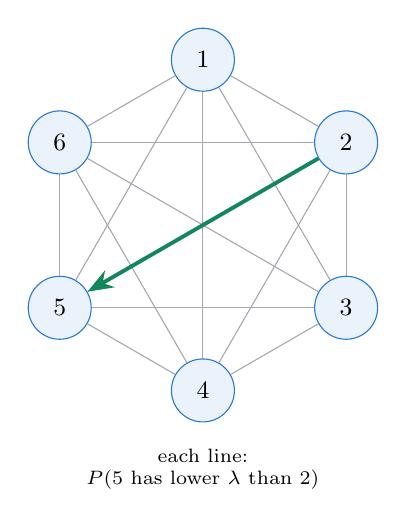
\begin{tikzpicture}
\foreach \a/\l in {90/1,30/2,-30/3,-90/4,-150/5,150/6} {\node[circle,draw=trace,fill=trace!10,minimum size=0.8cm,font=\small] (n\l) at (\a:2.1) {\l};}
\foreach \i/\j in {1/2,1/3,1/4,1/5,1/6,2/3,2/4,2/5,2/6,3/4,3/5,3/6,4/5,4/6,5/6} {\draw[ink2!50,visible on=<2->] (n\i)--(n\j);}
\draw[-{Stealth},model,line width=1.4pt,visible on=<3->] (n2)--(n5);
\node[font=\scriptsize,text width=3.5cm,align=center,visible on=<3->] at (0,-3.1) {each line: $P(\text{5 has lower }\lambda\text{ than 2})$};
\end{tikzpicture}}
\end{columns}
\end{frame}

\begin{frame}{Turning many pairwise verdicts into one order}
\eyebrow{Sorting algorithms}
Let $M_{ij}=\tfrac12\bigl(D_{ij}-D_{ji}\bigr)$, the predicted margin by which $i$ beats $j$ (both orders averaged).
\vspace{0.4em}
\begin{columns}[T]
\column{0.32\textwidth}
{\color{ink2}\bfseries mean change}\par\scriptsize
\[s_j=\tfrac{1}{n-1}\textstyle\sum_i M_{ij}\]
The least-squares ranking of the differences: uses the predicted \emph{sizes}. One large wrong prediction can move a screen far.
\column{0.32\textwidth}
{\color{ink2}\bfseries wins (round robin)}\par\scriptsize
\[s_j=\tfrac{1}{n-1}\textstyle\sum_i\mathrm{sign}\,M_{ij}\]
A tournament: count who beats whom. Robust to sizes, but a win over the worst screen counts as much as a win over the best.
\column{0.32\textwidth}
{\color{model}\bfseries Bradley--Terry (default)}\par\scriptsize
\[P(i\ \text{beats}\ j)=\frac{p_i}{p_i+p_j}\]
Each screen has a strength $p_i$, fitted to the (soft) wins. Beating a strong screen counts more. Score $=-\log p_i$.
\end{columns}
\vspace{0.6em}
\scriptsize\textbf{Fitting Bradley--Terry} (Hunter's MM algorithm): with soft wins $b_{ij}=\tfrac12+M_{ij}$ from the direction classifier,
\[p_i\ \leftarrow\ \frac{\sum_j b_{ij}+\tfrac12}{\sum_j\frac{1}{p_i+p_j}+\frac{1}{p_i+1}},\]
plus half a win against a virtual average opponent, so a screen that wins or loses everything keeps a finite score. Iterate to convergence; the board's score is the mean over its amplifiers (a setting applies to the whole board).
\end{frame}

\begin{frame}{Watching Bradley--Terry sort the first night}
\eyebrow{The sorting, iteration by iteration}
\begin{columns}[c]
\column{0.6\textwidth}\centering
\only<1| handout:0>{\fig{0.7\textheight}{figures/w_bt_iter0.png}}%
\only<2| handout:0>{\fig{0.7\textheight}{figures/w_bt_iter1.png}}%
\only<3| handout:0>{\fig{0.7\textheight}{figures/w_bt_iter2.png}}%
\only<4| handout:0>{\fig{0.7\textheight}{figures/w_bt_iter3.png}}%
\only<5| handout:1>{\fig{0.7\textheight}{figures/w_bt_iter4.png}}%
\column{0.38\textwidth}
\see{The 35 first-night settings as screens (new-amplifier models, $\lambda$ only). x: each setting's true rank. y: its Bradley--Terry score after 1, 2, 4, 11 and 60 MM iterations (step through the slides). Colour: the true $\lambda$ effect.}
\means{After the first iteration the order is already that of the soft-win counts (Spearman 0.84). Later iterations spread the scores out and count a win over a strong screen more than one over a weak screen (0.85 at convergence). The sort is fast and stable: the remaining scatter comes from the pairwise model, not from the sorting.}
\end{columns}
\end{frame}

\begin{frame}{The comparison matrix: the model's verdict on every pair}
\eyebrow{Inside the funnel}
\centering\fig[0.32\textwidth]{0.44\textheight}{figures/w_replay_matrix_truth.png}\hspace{1.5em}\fig[0.32\textwidth]{0.44\textheight}{figures/w_replay_matrix_model.png}\par\vspace{0.2em}
\begin{columns}[T]\column{0.485\textwidth}\see{$M_{ij}$ for the 35 settings (mean of the 3 amplifiers, new-amplifier models): blue = $i$ predicted to have lower $\lambda$ than $j$. Left: rows and columns ordered by the \emph{true} effect. Right: ordered by the model's score.}\column{0.485\textwidth}\means{Ordered by the truth, the top-right corner is blue and the bottom-left red: settings far apart in $\lambda$ are compared correctly. The middle is speckled: settings within the label noise of each other are close to coin flips. Ordered by the model's own score the pattern is smoother, because the many verdicts are largely \emph{consistent} with one order, which is what a sort needs. Single wrong verdicts are outvoted by the other 33.}\end{columns}
\end{frame}

\begin{frame}{The funnel replayed on the first night}
\eyebrow{Does the shortlist catch the best settings?}
\figright{0.66}{w_replay_scatter}
{Each dot is one of the 35 first-night settings: x = its true effect on $\lambda$ (vs nominal, drift removed, mean of 3 amplifiers), y = the Bradley--Terry score from traces only, with models that never saw that amplifier. Blue: the model's top 5. Green rings: the truly best 5.}
{The score follows the truth (Spearman 0.85). \textbf{3 of the 5 picks are among the truly best 5} (L1\_08, L1\_11, L1\_12, all $-16$\,\%). The single best setting (L1\_13, $-34$\,\%, far left) is ranked 7th, just outside the shortlist. The worst settings ($+50$ to $+140$\,\%) are never picked. This is one night and 35 settings, essentially \emph{one trial}. Session F (100 new settings, 5 picks vs 5 random controls) is the real test.}
\end{frame}

\begin{frame}{How many images do we need?}
\eyebrow{Regret}
\figright{0.6}{w_replay_regret}
{The $\lambda$ regret (how much worse the best imaged setting is than the truly best one) when imaging the model's top $k$ (blue) or $k$ random settings (grey, averaged over 3000 draws), first night.}
{Random picks need about 20 images to get within 7\,\% of the best. The model's first pick is already better than an average random one (32 vs 46\,\%). Its top 5 contain three settings 16\,\% below nominal (regret 18\,\% vs 21\,\% random: one outstanding setting, L1\_13, is missed), and its top 7 contain the best (regret 0 vs 18\,\%). \textbf{Regret} is the right score for a funnel: we do not need the whole order right, only the best inside the shortlist. Hence also: 5 picks is a choice, and 7--10 would be safer.}
\end{frame}

\begin{frame}{Comparing the ranking methods side by side}
\eyebrow{Which ranking?}
\figtop{0.42}{w_sorting_methods}
{Spearman with the true order of the 35 settings, for the objective weight $w$ (1:0 = $\sigma_e$ only, 0:1 = $\lambda$ only). Orange: with a nominal reference per screen (change model); grey: one-trace models; blue: screen vs screen with each sorting method; thick: Bradley--Terry.}
{For $\lambda$ (0:1), screen vs screen is best (0.84--0.85), ahead of the with-reference change model (0.64--0.76). For $\sigma_e$ (1:0) all methods are similar (0.67--0.84), and the good settings differ by only $\sim$3\,\%, so a $\sigma_e$ shortlist gains little. This is why the first round ranks on $\lambda$, without references, with Bradley--Terry.}
\end{frame}

\begin{frame}{The noise number attached to each pick}
\eyebrow{$\sigma_e$ for the shortlist}
\figright{0.66}{w_noise_attached}
{Predicted vs image $\sigma_e$ for every first-night row, from boosted trees on one trace's features plus the amplifier's name (5 packet folds). Band: the cross-validated typical error.}
{The funnel ranks on $\lambda$, then attaches this $\sigma_e$ prediction to each of the 5 picks (per amplifier and as the board mean), in the shortlist file and the changes-file comments. It never reorders the shortlist; it flags a pick whose noise would be unacceptable. On the funnel's own (trained) amplifiers it is good to about 10\,\%, enough to tell 0.15 from 0.20 e$^-$ but not to rank settings that differ by 3\,\%.}
\end{frame}

\begin{frame}{Later rounds: trading $\sigma_e$ against $\lambda$}
\eyebrow{The joint objective}
\[J(w)=w\,\Delta\log\sigma_e+(1-w)\,\Delta\log\lambda,\qquad 0\le w\le1,\quad\text{lower is better}\]
\begin{columns}[T]
\column{0.5\textwidth}\small
\begin{tabular}{lp{4.6cm}}\toprule
$w$ & meaning\\\midrule
1 : 0 & $\sigma_e$ only\\
0.5 : 0.5 & a given relative change of either counts the same\\
0 : 1 & $\lambda$ only (\textbf{first round})\\\bottomrule
\end{tabular}\par\medskip
\scriptsize The change model predicts $\Delta\log\sigma_e$ and $\Delta\log\lambda$ for every pair; $J$ combines them before sorting, so one model serves every weight.
\column{0.46\textwidth}\small
\textbf{Trade-offs.} A knob that lowers $\sigma_e$ but raises $\lambda$ is ranked by the weight. The alternative rule \textbf{``pareto''} puts the predicted Pareto front first (no setting predicted better in both) and orders within it by $J(w)$. On the first night it lost at the extremes, so \textbf{weighted} is the default.\par\medskip
\scriptsize The gain enters through $\sigma_e$ in electrons.
\end{columns}
\end{frame}

\begin{frame}{Where the funnel leads: levels 2 and 3}
\eyebrow{The full optimisation}
\begin{center}
\resizebox{\textwidth}{!}{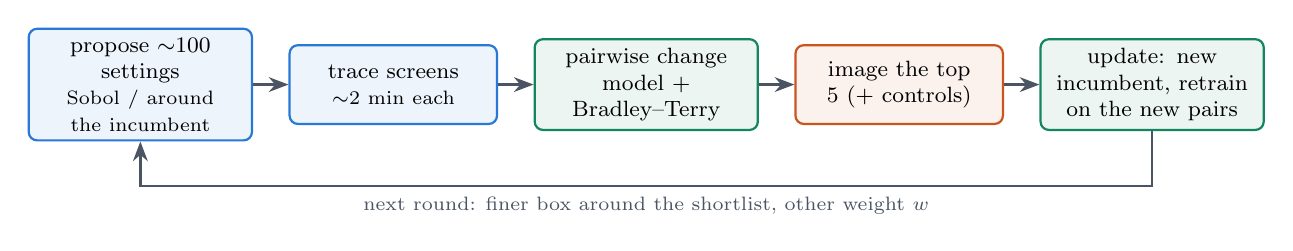
\begin{tikzpicture}[node distance=0.45cm]
\node[box=trace,text width=2.6cm,visible on=<1->] (a) {propose $\sim$100 settings\\\scriptsize Sobol / around the incumbent};
\node[box=trace,right=of a,text width=2.4cm,visible on=<2->] (b) {trace screens\\\scriptsize $\sim$2 min each};
\node[box=model,right=of b,text width=2.6cm,visible on=<3->] (c) {pairwise change model + Bradley--Terry};
\node[box=image,right=of c,text width=2.4cm,visible on=<4->] (d) {image the top 5 (+ controls)};
\node[box=model,right=of d,text width=2.6cm,visible on=<5->] (e) {update: new incumbent, retrain on the new pairs};
\draw[arr,visible on=<2->] (a)--(b); \draw[arr,visible on=<3->] (b)--(c); \draw[arr,visible on=<4->] (c)--(d); \draw[arr,visible on=<5->] (d)--(e);
\draw[arr,visible on=<6->] (e.south) -- ++(0,-0.7) -| node[pos=0.25,below,font=\scriptsize] {next round: finer box around the shortlist, other weight $w$} (a.south);
\end{tikzpicture}}
\end{center}
\vspace{0.6em}
\begin{columns}[T]
\column{0.32\textwidth}\scriptsize\textbf{Level 2:} a person runs the rounds: screens, shortlist, images, a finer box.
\column{0.32\textwidth}\scriptsize\textbf{Level 3:} the loop runs itself (preference-based Bayesian optimisation over the comparisons).
\column{0.32\textwidth}\scriptsize\textbf{Every round adds training pairs} on the very CCD being tuned, so the comparator gets better where it matters.
\end{columns}
\end{frame}

% ============================================================================================================
\divider{Step 7}{v2: what the next data taking is built to answer}{image!70}
\section{7 v2}

\begin{frame}{Every v2 change answers a first-night lesson}
\eyebrow[image]{From lessons to design}
\scriptsize
\begin{tabular}{p{5.6cm}p{6.6cm}}\toprule
first-night lesson & v2 change\\\midrule
one-knob packets made CV test extrapolation; C failed the CV choice & \textbf{joint Sobol design}: 12 knob groups move together, 38--48 levels each\\
$\lambda$ drifts 20\,\% a night; L1\_18 stalled with no flush & \textbf{flush before every image}; nominal every 7 packets\\
label noise known only at nominal & \textbf{3 replicates} of design points\\
96\,\% of within-packet $\sigma_e$ changes go up & \textbf{21 references at the previous packet's settings}\\
trace has no charge (gain) and misses the prescan/clear & \textbf{level-1 strips}: reference and new, read like the image\\
16 rows split dark current and CIC poorly & \textbf{32-row image}\\
3 C packets lost every trace & \textbf{checks on the spot}: retake damaged traces, restart a bad packet\\
learning curve still falling at 32 packets & \textbf{61 training packets} + 15 held out (session E)\\
the funnel needs testing on unseen settings & \textbf{session F}: 100 screens, 5 picks, 5 random controls\\\bottomrule
\end{tabular}
\end{frame}

\begin{frame}{Level-1 strips: a tiny image read exactly like the real one}
\eyebrow[image]{The new input}
\begin{columns}[T]
\column{0.5\textwidth}\small
\textbf{What it is.} $2\times1000$ pixels, 500 skips, after the same 5300-column prescan and register clear as the image, read at level 1: every skip's pedestal and signal sum of every pixel is kept ($\sim$16 MB per channel).\par\medskip
\textbf{Checked} on a 2026-10-06 L1 row: 80/80 pixels pass the layout checks, per-skip sd 5.37 ADU (traces 5.6).\par\medskip
\textbf{From it:} the strip's own \textbf{gain} (peak spacing, $\sim$1\,\%), \textbf{CIC + serial charge} ($\sim$5\,\%), $\sigma_e$, white noise, Allan curve.
\column{0.46\textwidth}
\resizebox{\linewidth}{!}{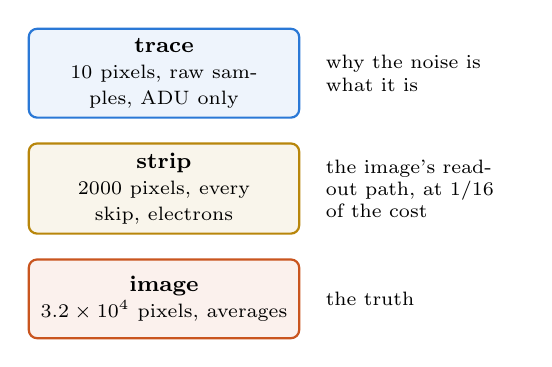
\begin{tikzpicture}[node distance=0.3cm]
\node[box=trace,text width=3.2cm,visible on=<1->] (t) {\textbf{trace}\\\scriptsize 10 pixels, raw samples, ADU only};
\node[box=gold,below=of t,text width=3.2cm,visible on=<2->] (s) {\textbf{strip}\\\scriptsize 2000 pixels, every skip, electrons};
\node[box=image,below=of s,text width=3.2cm,visible on=<1->] (i) {\textbf{image}\\\scriptsize $3.2\times10^4$ pixels, averages};
\node[right=0.2cm of t,font=\scriptsize,text width=2.4cm,visible on=<1->] {why the noise is what it is};
\node[right=0.2cm of s,font=\scriptsize,text width=2.4cm,visible on=<2->] {the image's readout path, at 1/16 of the cost};
\node[right=0.2cm of i,font=\scriptsize,text width=2.4cm,visible on=<1->] {the truth};
\end{tikzpicture}}
\end{columns}
\vspace{0.6em}
\scriptsize Three input sources on the same rows and folds: \textbf{traces}, \textbf{strip}, \textbf{both}. What does each predict, and do they add up? (Question Q1.)
\end{frame}

\begin{frame}{Why strips should fix the amplifier bias}
\eyebrow[image]{Measuring the level instead of guessing it}
\begin{columns}[T]
\column{0.52\textwidth}\small
\textbf{The problem (step 4).} A trace is in ADU; $\sigma_1^{\rm ADU}=\sigma_e\,g$ cannot be split, and the amplifier's level $c_a$ was only ever \emph{recognised}, not predicted. On a new amplifier the levels were lost.\par\medskip
\textbf{The strip resolves electrons}, so on \emph{this} amplifier, at \emph{these} settings, it measures
\[c_a\approx\log y_{\rm strip}(\theta)\quad\text{for gain, }\sigma_e,\ \text{CIC}.\]
The model then learns only the strip $\to$ image correction, which is about the readout path and not the amplifier's identity.
\column{0.44\textwidth}\small
\textbf{Evidence it works.} Board 102: every model's level was off, and \emph{one image} brought all of them to the label scatter. LOAO: with the offset removed, $\lambda$'s shape is learnt (28 vs 37\,\%).\par\medskip
\textbf{The strip is that ``one image''}, taken in every packet, at every setting, for 1/16 of the time.\par\medskip
\textbf{And for change models:} reference strip vs new strip gives a \emph{measured} within-packet change of gain and CIC, i.e.\ extra labels.
\end{columns}
\warnbox{\textbf{Limit:} strip rows barely wait, so the strip sees CIC and serial charge but only weakly the array dark current. $\lambda$'s array part still needs the image's rows (32 rows in v2).}
\end{frame}

\begin{frame}{The v2 packet}
\eyebrow[image]{Sequence}
\begin{center}
\resizebox{\textwidth}{!}{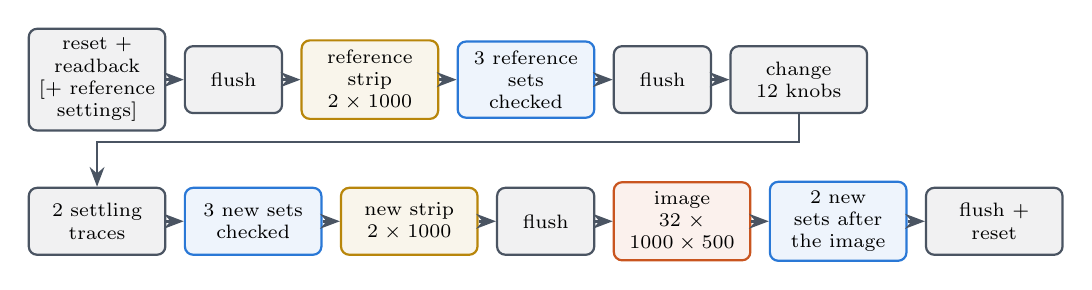
\begin{tikzpicture}[node distance=0.22cm]
\node[s,visible on=<1->] (a) {reset + readback\\{[}+ reference settings{]}};
\node[s,right=of a,text width=1.0cm,visible on=<1->] (b) {flush};
\node[s=gold,right=of b,visible on=<2->] (d) {reference strip\\$2\times1000$};
\node[s=trace,right=of d,visible on=<2->] (c) {3 reference sets\\checked};
\node[s,right=of c,text width=1.0cm,visible on=<3->] (e) {flush};
\node[s,right=of e,visible on=<3->] (f) {change\\12 knobs};
\node[s,below=0.7cm of a,visible on=<4->] (g) {2 settling traces};
\node[s=trace,right=of g,visible on=<4->] (h) {3 new sets\\checked};
\node[s=gold,right=of h,visible on=<5->] (i) {new strip\\$2\times1000$};
\node[s,right=of i,text width=1.0cm,visible on=<6->] (j) {flush};
\node[s=image,right=of j,visible on=<6->] (k) {image\\$32\times1000\times500$};
\node[s=trace,right=of k,visible on=<7->] (m) {2 new sets after the image};
\node[s,right=of m,visible on=<7->] (l) {flush + reset};
\foreach \x/\y/\v in {a/b/1,b/d/2,d/c/2,c/e/3,e/f/3,g/h/4,h/i/5,i/j/6,j/k/6,k/m/7,m/l/7} \draw[arr,visible on=<\v->] (\x)--(\y);
\draw[arr,visible on=<4->] (f.south) -- ++(0,-0.35) -| (g.north);
\end{tikzpicture}}
\end{center}
\vspace{0.4em}
\begin{columns}[T]
\column{0.32\textwidth}\scriptsize\textbf{Reference traces right before the change, new traces right after:} the two sides of a within-packet change are minutes apart; the strips bracket them.
\column{0.32\textwidth}\scriptsize\textbf{Traces bracket the image} (3 before, 2 after): drift of the trace across the image becomes visible.
\column{0.32\textwidth}\scriptsize\textbf{Checked on the spot}: damaged traces retaken; more than 5 restarts the packet. Every setting obeys the voltage relations (\texttt{ccd\_limits}).
\end{columns}
\end{frame}

\begin{frame}{A joint design covers the knob space, not just its axes}
\eyebrow[image]{Design}
\figtop{0.42}{w_design_coverage}
{Two projections of the settings: delayInt vs VR1 (left) and delay\_H vs VDD1 (right). Orange squares: the first night (sessions A--C). Blue dots: v2 sessions D and E (scrambled Sobol points, timing on a log scale). Star: nominal.}
{v1 moved one knob at a time (points on the lines through the star) plus 11 joint points. v2 fills the box, so every knob takes 38--48 values and combinations like ``delayInt and VR both changed'' appear in training as well as in the test. This turns the test into interpolation, gives the trees knobs they can split on, and gives the change models many ``two different kinds'' pairs.}
\end{frame}

\begin{frame}{The v2 plan: three sessions, 188 packets, about 28 hours}
\eyebrow[image]{Budget}
\figtop{0.36}{w_v2_budget}
{Packets (left) and hours (right) per session and purpose, from lvl1/packet\_plan\_v2/plan.json.}
{\textbf{D (training, 17.1 h):} 48 Sobol points, 10 nominal, 3 replicates; 21 references at the previous packet's settings. \textbf{E (held out, 4.3 h):} 12 new Sobol points + 3 nominal, scored once. \textbf{F (funnel, 6.9 h):} 100 trace-only screens, then the 5 shortlisted and 5 random-control images, nominal at both ends.}
\takeaway{one long night (D+E, 21.4 h) and a shorter one (F, 6.9 h). F needs the model trained on D+E between them: the shortlist packets stop run\_plan.sh until lvl1/funnel\_shortlist.py has written their settings.}
\end{frame}

\begin{frame}{From raw data to the funnel: where every piece of data goes}
\eyebrow[image]{Data flow}
\begin{center}
\resizebox{\textwidth}{!}{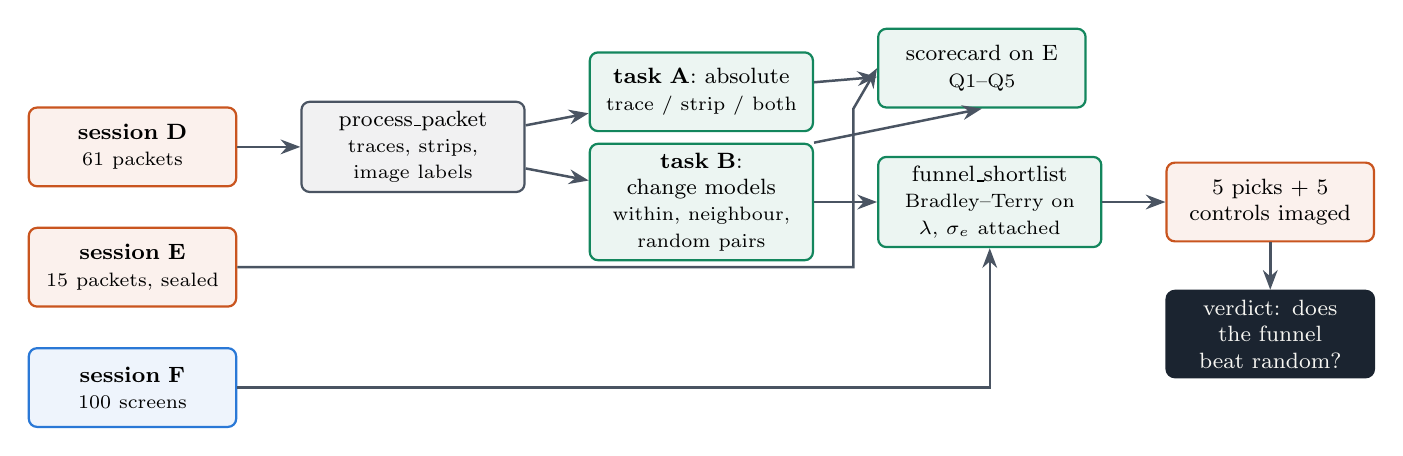
\begin{tikzpicture}[node distance=0.35cm]
\node[box=image,text width=2.4cm,visible on=<1->] (D) {\textbf{session D}\\\scriptsize 61 packets};
\node[box=image,below=0.5cm of D,text width=2.4cm,visible on=<1->] (E) {\textbf{session E}\\\scriptsize 15 packets, sealed};
\node[box=trace,below=0.5cm of E,text width=2.4cm,visible on=<4->] (F) {\textbf{session F}\\\scriptsize 100 screens};
\node[box,right=0.8cm of D,text width=2.6cm,visible on=<2->] (P) {process\_packet\\\scriptsize traces, strips, image labels};
\node[box=model,right=0.8cm of P,text width=2.6cm,yshift=0.7cm,visible on=<2->] (A) {\textbf{task A}: absolute\\\scriptsize trace / strip / both};
\node[box=model,right=0.8cm of P,text width=2.6cm,yshift=-0.7cm,visible on=<3->] (B) {\textbf{task B}: change models\\\scriptsize within, neighbour, random pairs};
\node[box=model,right=0.8cm of B,text width=2.6cm,visible on=<4->] (S) {funnel\_shortlist\\\scriptsize Bradley--Terry on $\lambda$, $\sigma_e$ attached};
\node[box=image,right=0.8cm of S,text width=2.4cm,visible on=<5->] (I) {5 picks + 5 controls imaged};
\node[box=model,right=0.8cm of A,text width=2.4cm,yshift=0.3cm,visible on=<6->] (R) {scorecard on E\\\scriptsize Q1--Q5};
\node[box=ink,fill=ink,text=paper,below=0.6cm of I,text width=2.4cm,visible on=<6->] (V) {verdict: does the funnel beat random?};
\draw[arr,visible on=<2->] (D)--(P); \draw[arr,visible on=<2->] (P)--(A); \draw[arr,visible on=<3->] (P)--(B);
\draw[arr,visible on=<4->] (B)--(S); \draw[arr,visible on=<4->] (F.east) -| (S.south); \draw[arr,visible on=<5->] (S)--(I);
\draw[arr,visible on=<6->] (E.east) -| ([xshift=-0.3cm]R.south west) -- (R.west); \draw[arr,visible on=<6->] (A)--(R); \draw[arr,visible on=<6->] (B.north east) -- (R.south); \draw[arr,visible on=<6->] (I)--(V);
\end{tikzpicture}}
\end{center}
\vspace{0.3em}
\scriptsize Session D trains and chooses the models; E is opened once to score them (the honest test); F tests the funnel on 100 settings no model has seen. The images of the 10 F picks also become new labelled data.
\end{frame}

\begin{frame}{What v2 should answer, and what we do with each answer}
\eyebrow[image]{Questions and decisions}
\scriptsize
\begin{tabular}{p{5.4cm}p{7.2cm}}\toprule
question & if yes / if no\\\midrule
\textbf{Q1} which cheap measurement predicts the image: traces, strip, or both? & strip for gain and $\lambda$ levels, traces for $\sigma_e$; or traces alone if they suffice\\
\textbf{Q2} is the change between any two traces predicted, in size or only in direction? & size: level 2 regresses; direction only: preference-based optimisation\\
\textbf{Q3} does it carry over to a new amplifier / CCD? & build level 2 on the trace models / per-CCD calibration session\\
\textbf{Q4} is more data still helping at 61 packets? & take a third (longer) night\\
\textbf{Q5} how good are the labels at every setting? & set the clear-change thresholds and the weights of the direction classifier\\
\textbf{F} do the 5 picks image clearly better than the 5 controls? & level 2 screens with traces and images only the shortlist / images for every candidate\\\bottomrule
\end{tabular}
\vspace{0.5em}
\takeaway{level 1 passes if, on session E, the trace (alone or with the strip) predicts $\sigma_e$ and $\lambda$ significantly better than the no-trace references, within about twice the label scatter, and gets the direction of clear changes right at least 85\,\% of the time on amplifiers not in training.}
\end{frame}

\begin{frame}{What more data will (and will not) fix}
\eyebrow[image]{Expectations}
\begin{columns}[T]
\column{0.48\textwidth}\small
{\color{model}\bfseries More data should help}\par\scriptsize
\begin{itemize}
\item $\sigma_e$ and $\lambda$ errors: still falling at 32 packets (learning curve).
\item Significance: the scorecard's relative cells had $\sim$50 clear changes each; v2's random pairs give thousands.
\item ``Two different kinds'' comparisons: the case level 2 needs and v1 has 48 pairs of.
\item Clock rails, VSUB: almost no clear changes in v1, now moved jointly with the rest.
\item Ranking: the first-night ranking was $\sim$one trial (3 amplifiers share settings); F is a new, independent trial.
\end{itemize}
\column{0.48\textwidth}\small
{\color{problem}\bfseries More data will not fix}\par\scriptsize
\begin{itemize}
\item The amplifier's level from a trace alone: a physical degeneracy ($\sigma_e\,g$), not a sample-size problem. Strips or one calibration image fix it.
\item $\lambda$'s history dependence: needs the fixed pre-image routine and the drift tracking, not more packets.
\item A second CCD: transfer can only be tested on a CCD whose settings are varied too.
\end{itemize}
\end{columns}
\end{frame}

\begin{frame}{Summary}
\eyebrow[model]{Conclusions and why}
\scriptsize
\begin{tabular}{p{6.2cm}p{6.6cm}}\toprule
conclusion & because\\\midrule
the trace predicts the image's $\lambda$ (5.3\,\% on C) and $\sigma_e$ (7.3\,\%) on known amplifiers & sealed session C, vs 23\,\% / 10\,\% without a trace\\
physics-structured models generalise, flexible ones extrapolate badly & CV on one-knob packets ranked them wrong; C reversed it\\
the amplifier's level is recognised, not predicted & fingerprints ($\eta^2$), LOAO, board 102, gain = $\sigma_e\,g$\\
differences cancel the level: change models transfer & on ch2, absolute models miss by 54--100\,\%, change models by at most 7\,\%\\
for ranking, a direction classifier on [A, B, B$-$A] with random pairs is best & Spearman 0.85 on a new amplifier ($\lambda$)\\
screen vs screen + Bradley--Terry sorts 35 settings from traces alone & first-night replay; reference traces add nothing\\
v2: joint design, strips, more and checked data, funnel test & each fixes a specific first-night failure\\\bottomrule
\end{tabular}
\vspace{0.5em}
\takeaway{the realistic level-1 product is a comparator: ``is setting B better than A for this amplifier?'' from two short traces, plus one measured level per amplifier (strip or image). That is exactly what the funnel, and level 2 after it, needs.}
\end{frame}

{\setbeamercolor{background canvas}{bg=ink}\setbeamertemplate{footline}{}
\begin{frame}[plain]
\vfill
{\color{trace!60}\small\bfseries WHERE EVERYTHING IS}\par\vspace{0.8em}
{\color{paper}\tiny
\begin{tabular}{ll}
first-data report & docs/overleaf\_first\_data\_2026-11-03/first\_data.pdf\\
level-1 summary & docs/overleaf\_overview\_2026-11-04/level1\_summary.pdf\\
scorecard, relative models, rankings & docs/scorecard\_2026-11-04/ (lvl1/scorecard.py, relative\_extra.py, rank\_methods.py)\\
funnel & lvl1/funnel\_shortlist.py, lvl1/shortlist.py; replay: lvl1/funnel\_replay.py\\
v2 plan & docs/overleaf\_v2\_training\_plan\_2026-11-04/v2\_training\_plan.pdf, lvl1/packet\_plan\_v2/\\
this deck's figures & docs/slides/make\_walkthrough\_2026\_11\_05.py\\
running log & docs/context/2026-11-03\_session\_context.md
\end{tabular}}
\vfill
\end{frame}}

\end{document}
